\documentclass{article}

\usepackage[T1]{fontenc}
\usepackage[utf8]{inputenc}
\usepackage[brazilian]{babel}
\usepackage{graphicx}
\usepackage[export]{adjustbox}[2011/08/13]
\usepackage{float}
\usepackage[pdftex]{hyperref}
\usepackage{epstopdf}
\usepackage{etoolbox}
\usepackage{amsmath}
\usepackage{amsfonts}
\usepackage{amssymb}
\usepackage{caption}
\usepackage{subcaption}
\usepackage{setspace}
\usepackage{tikz}
\usepackage{listings}
\usepackage{xcolor} 

\bibliographystyle{eric}
\patchcmd{\thebibliography}{\section*}{\section}{}{}


\newcommand{\R}{\ensuremath{\mathbb{R}}}
\newcommand{\Prob}{\ensuremath{\mathbb{P}}}
\newcommand{\K}{\ensuremath{\mathbb{K}}}
\newcommand{\U}{\ensuremath{\mathbb{U}}}
\newcommand{\N}{\ensuremath{\mathbb{N}}}
\newcommand{\Lg}{\ensuremath{\mathbb{L}}}
\newcommand{\T}{\ensuremath{\rm Tr}}
\newcommand{\sg}{{\sigma(x_k)}}

\newcommand{\G}{\ensuremath{\mathcal{G}}}
\newcommand{\F}{\ensuremath{\mathcal{F}}}
\newcommand{\C}{\ensuremath{\mathcal{C}}}
\newcommand{\E}{\ensuremath{\mathcal{E}}}
\newcommand{\Hn}{\ensuremath{\mathcal{H}}}
\newcommand{\Hoo}{\ensuremath{\mathcal{H}_\infty}}
\newcommand{\Hop}{\ensuremath{\mathcal{H}_{op}}}
% --------------------------------------------------
\newtheorem{theo}{Teorema}
\newtheorem{exa}{Exemplo}
\newtheorem{lemm}{Lema}
\newtheorem{coro}{Corolário}
\newtheorem{defn}{Definição}[section]

\begin{document}
\input{capa.tex}

\onehalfspacing
\section{Objetivos}
	Este projeto tem como objetivo realizar o acionamento de um motor DC utilizando conversor de potência, controlar a posição por meio de servo-acionamento, e integrar componentes elétricos e mecânicos por malha de controle. 

\section{Motor e Conversor de Potência}
Implementamos no Simulink o circuito apresentado na figura \ref{fig:sim1}. Configuramos o bloco do motor DC disponível para que atuasse como motor DC de ímãs permanentes. Definimos os parâmetros do motor conforme especificado na tabela \ref{tab:param}. Determinamos o torque nominal do motor utilizando a equação \ref{eq:torque} e a constante de torque/corrente de armadura nominal resolvendo as equações \ref{eq:m1} e \ref{eq:m2}. Existem duas combinações possíveis de constante de torque e corrente nominal que atingem os pré requisitos, escolhemos a menor corrente.

\begin{equation}
	\label{eq:torque}
	T_{nom} = \frac{P_{nom}}{\omega_{nom}}
\end{equation}

\begin{equation}
\label{eq:m1}
	V_{nom} = R_a*I_{nom} + k_t*\omega_{nom}
\end{equation}

\begin{equation}
	\label{eq:m2}
	T_{nom} = k_t*I_{nom}
\end{equation}


\begin{figure}[H]
	\centering
	\includegraphics[width=\linewidth]{matlab/sim1}
	\caption{Esquemático da simulação para dimensionamento do motor DC e conversor}
	\label{fig:sim1}
\end{figure}

\begin{table}[]
	\centering
	\caption{Parâmetros do motor DC}
	\label{tab:param}
	\begin{tabular}{|c|c|}
		\hline
		\textbf{Parâmetro}              & \textbf{Valor}                 \\ \hline
		Potência nominal                & $5\ HP$                        \\ \hline
		Velocidade nominal              & $1750\ rpm$                    \\ \hline
		Tensão nominal                  & $240\ V$                       \\ \hline
		Torque nominal					& $20.3455\ Nm$ \\ \hline
		Corrente nominal				& $19.7128\ A$ \\ \hline
		Resistência de armadura ($R_a$) & $2,58\ \Omega$                 \\ \hline
		Indutância de armadura ($L_a$)  & $28\ mH$                       \\ \hline
		Inércia ($J$)                   & $2,22 \times 10^{-2}\ kg\ m^2$ \\ \hline
		Atrito viscoso ($B$)            & $2,95 \times 10^{-3}\ N\ m\ s$ \\ \hline
		Constante de Torque ($k_t$)		& $1.0321\ Nm/A$ \\ \hline
	\end{tabular}
\end{table}

Para o acionamento do motor, utilizamos uma ponte H composta por MOSFETs, sendo que o circuito de acionamento funciona com a diferença de potencial entre sinal de controle ($v_{cont}$) e uma onda triangular ($v_{tri}$), com funcionamento explicado pela figura \ref{fig:ponte}. Para fins de simulação utilizamos $v_{cont}$ e $v_{tri}$ variando entre $0\ V$ e $100\ V$, mas este valor pode variar desde que atenda aos requisitos de acionamento do MOSFET.

\begin{figure}[H]
	\centering
	\begin{subfigure}[t]{0.45\textwidth}
		\includegraphics[width=\linewidth]{ponte1}
		\caption{Controle e onda triangular}
	\end{subfigure}
	\begin{subfigure}[t]{0.45\textwidth}
		\includegraphics[width=\linewidth]{ponte2}
		\caption{Duty cycle e tensão de saída}
	\end{subfigure}
	\caption{Esquema de funcionamento do circuito de controle da ponte H}	
	\label{fig:ponte}
\end{figure}

A fim de garantir um bom fator de forma na saída do conversor, colocamos um capacitor de filtro $C_f$ em paralelo com a carga. Para o motor em questão chegamos ao seguinte valor:

\begin{equation}
C_f=1000\ \mu F
\end{equation}

Fizemos a simulação da resposta do motor a um degrau com $V_{out}=240\ V$, sem cargas, apenas com os parâmetros físicos definidos nele mesmo.
Obtivemos os resultados de tensão e correntes de armadura ($v_a$ e $i_a$), e também curvas de torque e velocidade angular ($T_{em}$ e $\omega_m$) conforme figura \ref{fig:sim1viwt}.

\begin{figure}[H]
	\centering
	\begin{subfigure}{0.45\textwidth}
		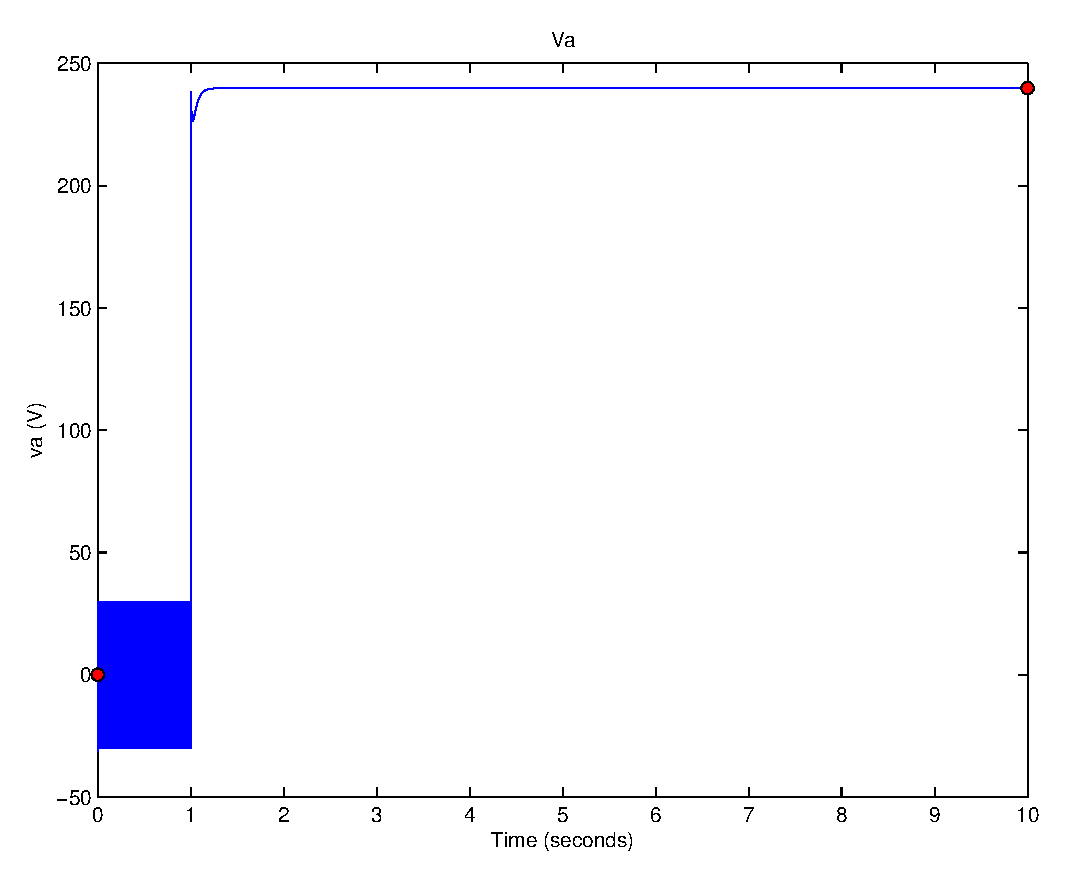
\includegraphics[width=\linewidth]{matlab/va1}
		\caption{Tensão de armadura}
	\end{subfigure}
	\begin{subfigure}{0.45\textwidth}
		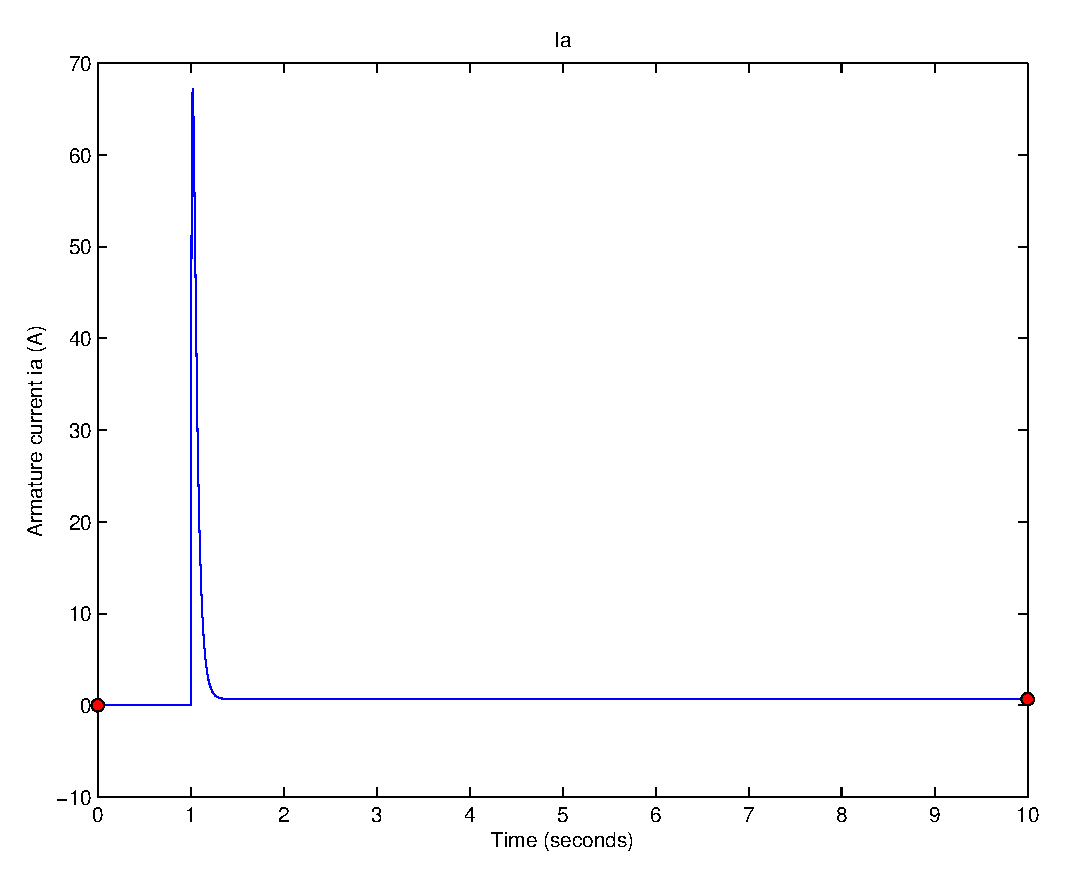
\includegraphics[width=\linewidth]{matlab/ia1}
		\caption{Corrente de armadura}
	\end{subfigure}
	\begin{subfigure}{0.45\textwidth}
		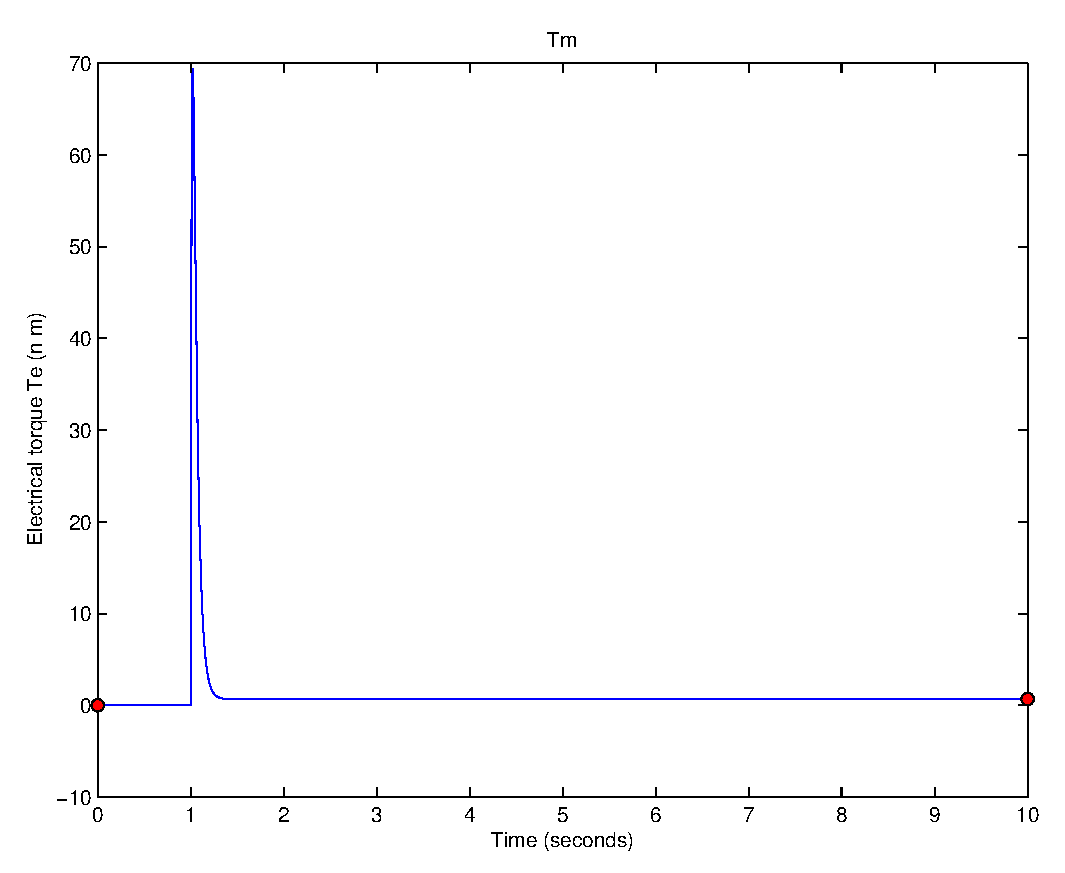
\includegraphics[width=\linewidth]{matlab/tm1}
		\caption{Torque}
	\end{subfigure}
	\begin{subfigure}{0.45\textwidth}
		\includegraphics[width=\linewidth]{matlab/wm1}
		\caption{Velocidade angular}
	\end{subfigure}
	\caption{Resposta ao degrau de $240\ V$ no motor DC}	
	\label{fig:sim1viwt}
\end{figure}

Podemos ver que ainda existe uma oscilação significativa na tensão de armadura, porém julgamos inviável aumentar a capacitância de filtro. Notamos também que a velocidade atingida supera a velocidade nominal, fator esperado uma vez que estamos trabalhando sem carga. Existe um pico de corrente que ultrapassa significativamente o valor nominal e que pode vir a danificar o motor.

\section{Servo-acionamento}
Iniciamos o projeto do servo-acionamento pelo controle PI de corrente. Utilizando o Simulink, conforme figura \ref{fig:sim2}.

\begin{figure}[H]
	\centering
	\includegraphics[width=\linewidth]{matlab/sim2}
	\caption{Esquemático da simulação do controlador de corrente}
	\label{fig:sim2}
\end{figure}

Para facilitar o controle somamos um offset de $50\%$ no duty-cycle de saída, assim se o esforço de controle for negativo a tensão sobre o motor será negativa e se este for positivo a tensão será positiva. Dimensionamos o controlador PI para que ele responda a um degrau unitário com erro estacionário de menos de $0,2\ A$ e com tempo de resposta menor do que $100\ ms$. Para isso escolhemos as constantes proporcional e integral de maneira iterativa, ajustando-as de para atingir nosso objetivo. As constantes escolhidas foram:
\begin{equation}
	k_p = 3
\end{equation}
\begin{equation}
	k_i = 100
\end{equation}

A resposta do controlador ao degrau unitário está apresentada na figura \ref{fig:ia2}, podemos ver que ele tem uma resposta satisfatória considerando os requisitos de projeto.
\begin{figure}[H]
	\centering
	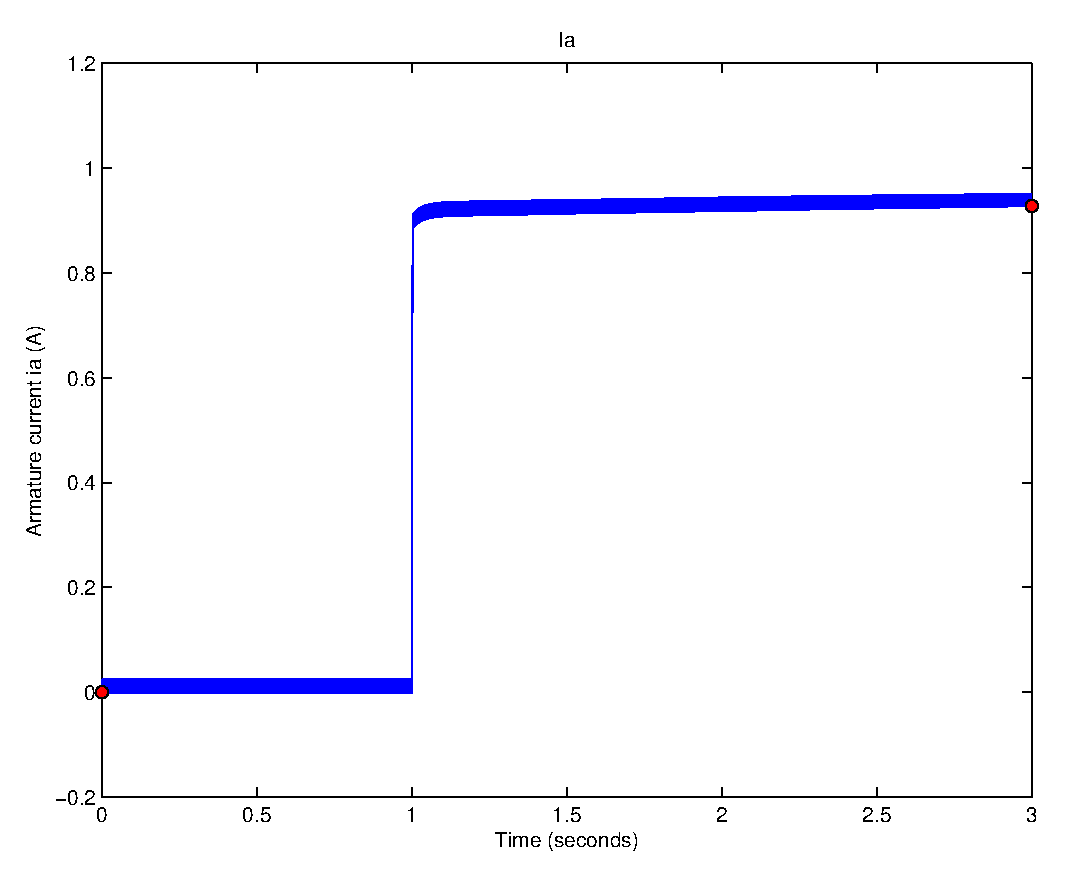
\includegraphics[width=0.7\linewidth]{matlab/ia2}
	\caption{Resposta do controlador de corrente ao degrau unitário}
	\label{fig:ia2}
\end{figure}

\section{Modelagem do Manipulador}
\section{Acoplamento Motor-Robô}


\bibliography{mybib}
\end{document}

